\section{Shortcomings}

None of our proposed algorithms were able to achieve any meaningful reduction from Always Full Mark's number of false positives. As a result, we investigated potential sources of error that may have been been caused by our assumptions.

\subsection{Too Much Noise in Edit Distance}
\label{sec:ctm-too-much-noise}

One of the underlying assumptions that our tool made was that the edit distance we compute must accurately reflect the closeness of two program files. Although we tried encapsulating structural differences into a tree edit distance and ensuring logically similar code had low edit distances, the edit difference was still ultimately a scalar value that discarded potentially useful information.

When we manually inspected a couple of assignments marked as false positives (assignments that were automated to higher marks than they had earned from human markers), we noticed some of them had glaring issues that were not penalized as heavily relative to the overall edit distance. For example, one student did not use the Pthread library at all for the Parallel Processing assignment and thus should had failed. However, our tool only penalized  an edit distance of 100 for inserting the appropriate \texttt{CallStatement} nodes whereas final edit distances were normally between 500 to 800. As a result, this catastrophic failure went undetected as it got treated as a small outlier. This problem might had been caught if the penalty was magnitudes higher (e.g. \num{10000}). However, this might also obscure other issues because it would be magnitudes larger than other penalties.

Overall, we believe the single scalar value has too much noise to make accurate predictions. There are several avenues to pursue to improve this step: prune more unnecessary nodes from the ASTs, adjust the cost model penalties for key function calls, or generate a multi-dimensional matrix to represent program differences and to be used as input to our aggregator.

\subsection{Uncertain Ground-Truth}
\label{sec:ctm-uncertain-ground-truth}

There was some uncertainty in our ground-truth for the students' actual marks. Historical mark breakdowns were not archived and thus the marks we used include non-technical deductions such as issues with the student's written report, late submissions, or plagiarism. In addition, there was a discrepancy in marker leniency between the two years, as seen in Figure~\ref{fig:ctm-marker-discrepancy}. As a result, the \textquote{true} student marks that we used to measure our accuracy were not as reliable as we originally assumed.

\begin{figure}
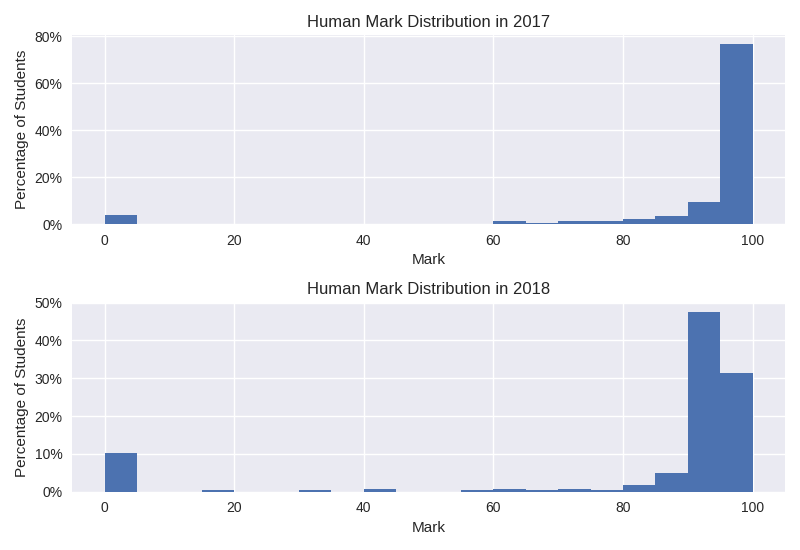
\includegraphics[width=\textwidth]{human_marks}
\caption[Marker Discrepancy Between 2017 and 2018]{There is a discrepancy in marker leniency between 2017 and 2018. Since markers change every semester, the two classes had different markers. In the 2017 class, about 80\% of the class received a 95 or higher from the marker whereas in the 2018 class, only 35\% of the class received a 95 or higher from the marker.}
\label{fig:ctm-marker-discrepancy}
\end{figure}

To verify whether the uncertainties in our ground-truth had a significant impact on our results in Section~\ref{sec:ctm-results}, we randomly selected 20 students from each class and remarked their assignments to ensure accuracy and consistency. Tables~\ref{tab:ctm-remarked-w2017} and \ref{tab:ctm-remarked-w2018} present the automation and false positive rates of our sampled students with their re-evaluated marks. Since we changed the ground-truth, only the false positive rate should change. However we still present the automation rate to verify that our random sample is representative of their entire class. This was indeed the case as we see that the automation rate was roughly identical to the automation rates of the entire class presented Figure~\ref{fig:ctm-results}; Gaussian Mixture had the highest automation rate while the others fell behind with HDBSCAN as the lowest.

When we compare the false positive rates, we see that Gaussian Mixture (the algorithm we initially observed to be strictly worse than the  baseline Always Full Marks) had a slightly better result than the baseline for both classes. In the 2017 class, Gaussian Mixture had zero false positives whereas the baseline had two false positives. Due to our small sample size and the fact that we were only able to automate 40\% of the students, this might had simply been a coincidence. However when we look at the 2018 class, we see that Gaussian Mixture was able to automate 70\% of the students with 21\% false positive rate compared to Always Full Marks at 35\% false positive rate.

Despite having a lower false positive rate than our baseline, 21\% is still too high to be considered usable in a live-classroom environment. Nonetheless, this sample has demonstrated promising potential in our tool to perform better than blindly assigning everyone full marks. Further refinements to our tool may eventually lead to a false positive rate low enough to be considered usable in a regular classroom.

\begin{table}
\caption{Automated Marks With New Ground-Truth for Class of 2017}
\label{tab:ctm-remarked-w2017}
\begin{tabular}{lrrrr} \toprule
\multirow{2}{*}{}
& \multicolumn{2}{c}{90 Cutoff} & \multicolumn{2}{c}{95 Cutoff}  \\
& Automated & False Positives & Automated & False Positives  \\
\midrule
Always Full Marks & 20 & 2 & 20 & 2 \\
Minimum Distance  & 5  & 0 & 5  & 0 \\
K-Means           & 2  & 0 & 2  & 0 \\
Gaussian Mixture  & 8  & 0 & 8  & 0 \\
HDBSCAN           & 0  & - & 0  & - \\
\bottomrule
\end{tabular}

\caption{Automated Marks With New Ground-Truth for Class of 2018}
\label{tab:ctm-remarked-w2018}
\begin{tabular}{lrrrr} \toprule
\multirow{2}{*}{}
& \multicolumn{2}{c}{90 Cutoff} & \multicolumn{2}{c}{95 Cutoff}  \\
& Automated & False Positives & Automated & False Positives  \\
\midrule
Always Full Marks & 20 & 7 & 20 & 7 \\
Minimum Distance  & 1  & 0 & 1  & 0 \\
K-Means           & 2  & 0 & 2  & 0 \\
Gaussian Mixture  & 14 & 3 & 14 & 3 \\
HDBSCAN           & 0  & - & 0  & - \\
\bottomrule
\end{tabular}
\end{table}
